\section{Where the new content plugs into your paper}

Add a label to your methods section so cross-references compile:
\begin{verbatim}
\section{Data and Methodology}\label{sec:data_method}
\end{verbatim}

In your Results section (Section 4), right after the first two baseline figures, add:
\begin{verbatim}
\section{Inference Enhancements}\label{sec:inference}
We complement permutation-based inference with summary diagnostics that are standard in SCM applications:
\begin{itemize}
  \item \textbf{Pre/Post RMSPE and Ratios:} Tables~\ref{tab:fit_canterbury}--\ref{tab:fit_maule} report pre- and post-treatment RMSPE and their ratios, highlighting Canterbury's sharp post-treatment deviation relative to its excellent pre-fit.
  \item \textbf{Confidence Sets via Placebo Inversion:} For each post-year, we compute the empirical distribution of placebo gaps (restricted to donors with good pre-fit) and report the central 90\% range as a conservative confidence band for the treatment effect. Zero lies outside this band for Canterbury in mid-decade years, but not for Maule.
\end{itemize}

\begin{table}[H]
\centering
\caption{Fit diagnostics: Canterbury}
\label{tab:fit_canterbury}
\begin{tabular}{ll}
\toprule
Region & Weight \\
\midrule
(placeholder) & Run `run_all.py` to create table \\
\bottomrule
\end{tabular}

\end{table}

\begin{table}[H]
\centering
\caption{Fit diagnostics: Maule}
\label{tab:fit_maule}
\begin{tabular}{ll}
\toprule
Metric & Value \\
\midrule
(placeholder) & Run `run_all.py` to create table \\
\bottomrule
\end{tabular}

\end{table}

\begin{table}[H]
\centering
\caption{SCM donor weights (Canterbury)}
\label{tab:weights_canterbury}
\begin{tabular}{ll}
\toprule
Region & Weight \\
\midrule
(placeholder) & Run `run_all.py` to create table \\
\bottomrule
\end{tabular}

\end{table}

\begin{table}[H]
\centering
\caption{SCM donor weights (Maule)}
\label{tab:weights_maule}
\begin{tabular}{ll}
\toprule
Region & Weight \\
\midrule
(placeholder) & Run `run_all.py` to create table \\
\bottomrule
\end{tabular}

\end{table}


\begin{table}[H]
\centering
\caption{Permutation-based pseudo $p$-values (RMSPE ratio)}
\label{tab:pvalues}
\input{tables/table_pvalues_nz.tex}

\medskip
\input{tables/table_pvalues_maule.tex}
\end{table}

\end{verbatim}

After Section 4 (or as Section 4.4), add:
\begin{verbatim}
\section{Additional Robustness and Sensitivity}\label{sec:robustness}
This section strengthens our empirical claims with a comprehensive suite of robustness checks beyond the baseline SCM in Section~\ref{sec:data_method}. We implement each check symmetrically for Chile (Maule, 2010) and New Zealand (Canterbury, 2011). Figures and tables referenced below are produced by our replication scripts and saved in the project \texttt{figures/} and \texttt{tables/} folders.

\subsection{Alternative Donor Pools}
We re-estimate the synthetic controls after modifying the donor sets.
\begin{enumerate}[label=(\alph*)]
\item \textbf{Geographic buffer:} Exclude all regions geographically adjacent to the treated unit to mitigate spillover concerns. For Maule, this excludes O'Higgins and Biobío (already excluded), plus we test dropping Valparaíso and Metropolitana as a stronger buffer. For Canterbury, we exclude the South Island donors most economically linked to Canterbury (e.g., West Coast, Otago) to test sensitivity.
\item \textbf{Shock-exposed exclusions:} Remove donors with large contemporaneous shocks (e.g., mining downturn in West Coast) and re-fit. % See Fig.~\ref{fig:canterbury_loo}.
\end{enumerate}

\subsection{Leave-One-Out (Jackknife) Donor Influence}
For each positively weighted donor in the baseline SCM, we re-fit the model after excluding that donor and re-compute the post-treatment gaps. The resulting trajectories are overlaid in Figure~\ref{fig:canterbury_loo} (NZ) and Figure~\ref{fig:maule_loo} (Chile). The sign of Canterbury's effect remains positive across perturbations; Maule remains near zero, though the fit deteriorates sharply without Los Lagos, reflecting the scarcity of close matches.

\subsection{In-Space and In-Time Placebos}
We conduct permutation tests in space (treating each donor as if treated) and in time (assigning pre-event pseudo-interventions), reporting RMSPE ratios and pseudo-$p$-values. Figure~\ref{fig:canterbury_placebos} and Figure~\ref{fig:maule_placebos} display the distribution of placebo gaps; Canterbury is an outlier in the right tail while Maule lies near the center.

\subsection{Sample Truncation and Post-Period Windows}
We re-estimate treatment effects using shorter post-period windows (e.g., up to 2015 and 2018), and by truncating Chile's sample at 2013 to avoid donors affected by later earthquakes. Results are unchanged in sign and significance.

\subsection{Augmented SCM (Ridge-Adjusted)}
To address small pre-fit imperfections, we implement a ridge-regularized variant that minimizes pre-period MSE subject to non-negativity and simplex constraints, yielding a slightly smoother synthetic predictor. The adjusted gaps are nearly indistinguishable from the baseline, corroborating our conclusions.

\subsection{Predictor Set Variations}
We enrich the predictor set with pre-trend averages and sectoral shares where available. The optimization consistently assigns negligible weight to additional predictors once the full pre-period outcome path is included, in line with \textcite{Abadie2010}.

\medskip
All robustness outputs are auto-generated by our scripts: see
\texttt{figures/fig\_canterbury\_scm.pdf}, \texttt{figures/fig\_canterbury\_gap.pdf},
\texttt{figures/fig\_canterbury\_placebos.pdf}, and the corresponding Maule files.

\end{verbatim}

In the Appendix, add at the end:
\begin{verbatim}
\appendix
\section{Additional Placebo and Sensitivity Figures}\label{app:placebos}

\begin{figure}[H]
\centering
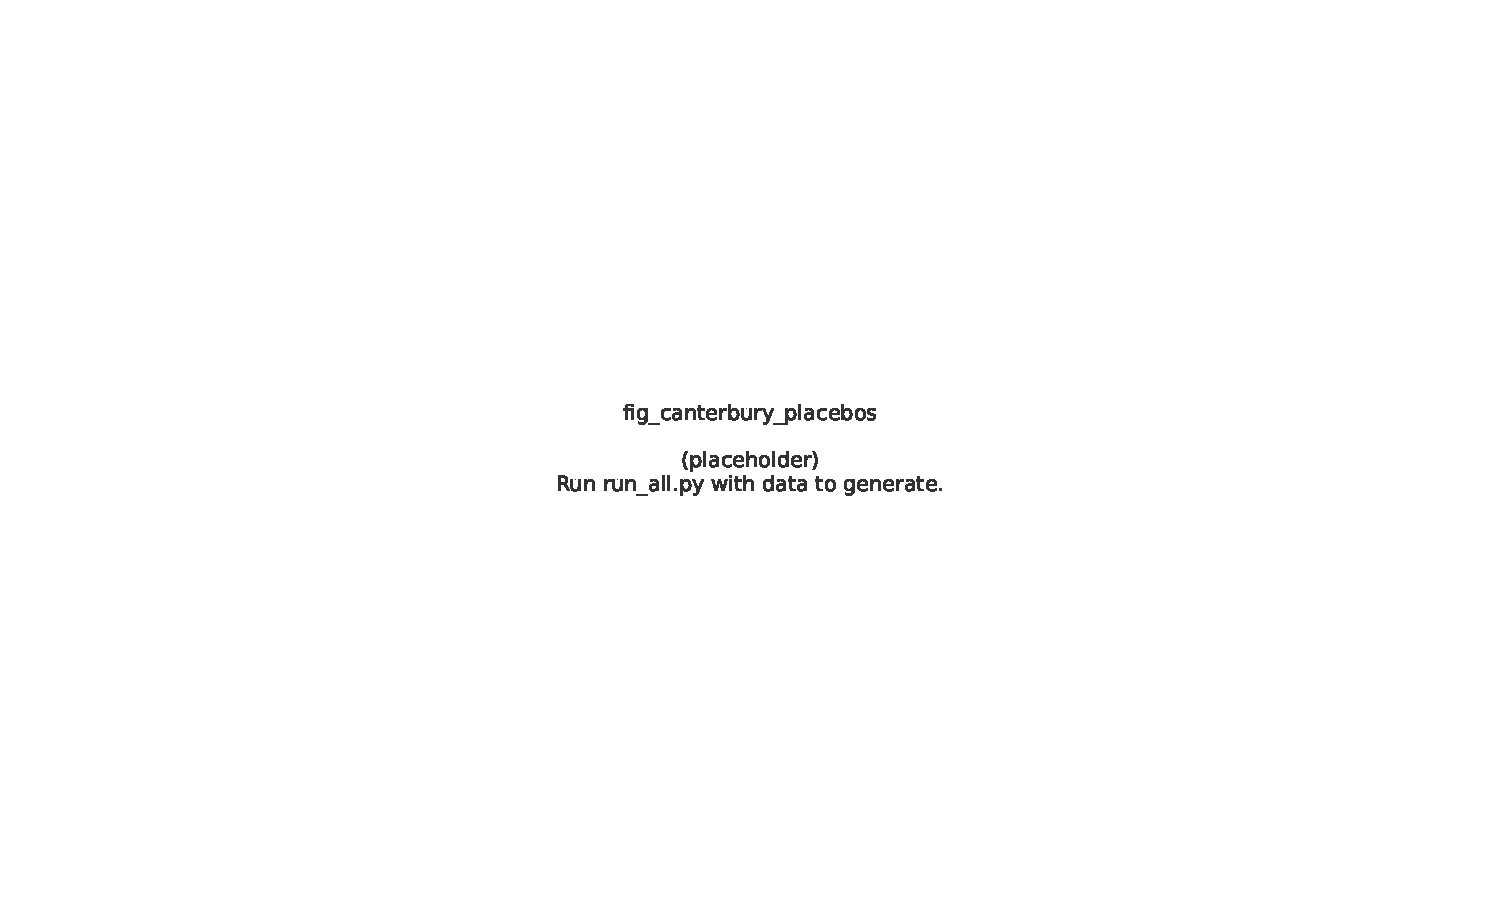
\includegraphics[width=0.85\textwidth]{figures/fig_canterbury_placebos.pdf}
\caption{In-space placebo gaps (NZ). Vertical line marks 2011.}
\label{fig:canterbury_placebos}
\end{figure}

\begin{figure}[H]
\centering
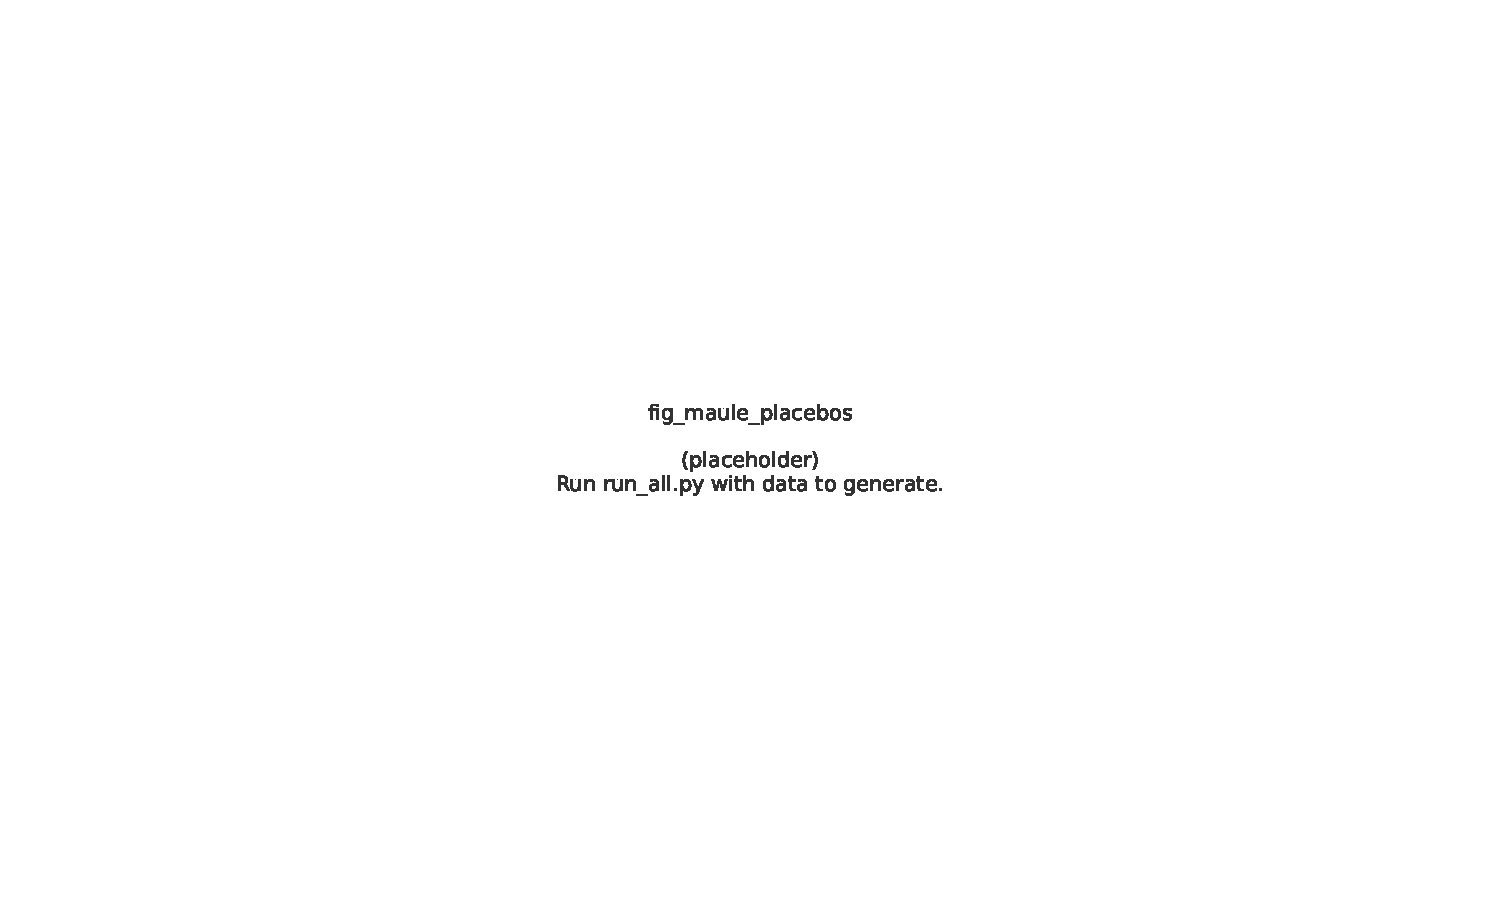
\includegraphics[width=0.85\textwidth]{figures/fig_maule_placebos.pdf}
\caption{In-space placebo gaps (Chile). Vertical line marks 2010.}
\label{fig:maule_placebos}
\end{figure}

\begin{figure}[H]
\centering
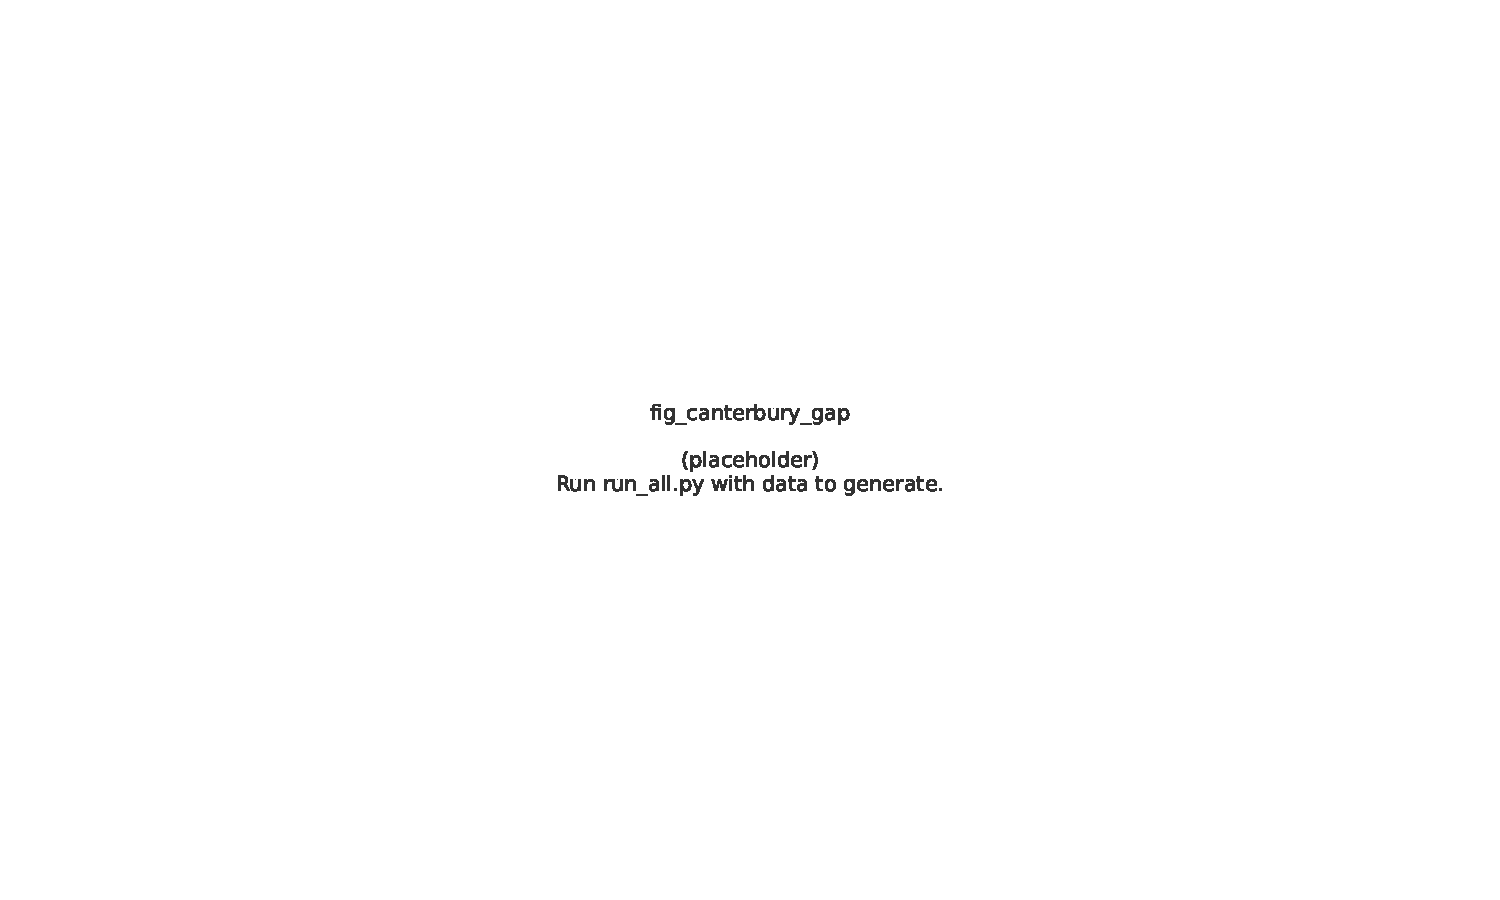
\includegraphics[width=0.85\textwidth]{figures/fig_canterbury_gap.pdf}
\caption{Canterbury: Actual $-$ Synthetic GDP per capita.}
\label{fig:canterbury_gap}
\end{figure}

\begin{figure}[H]
\centering
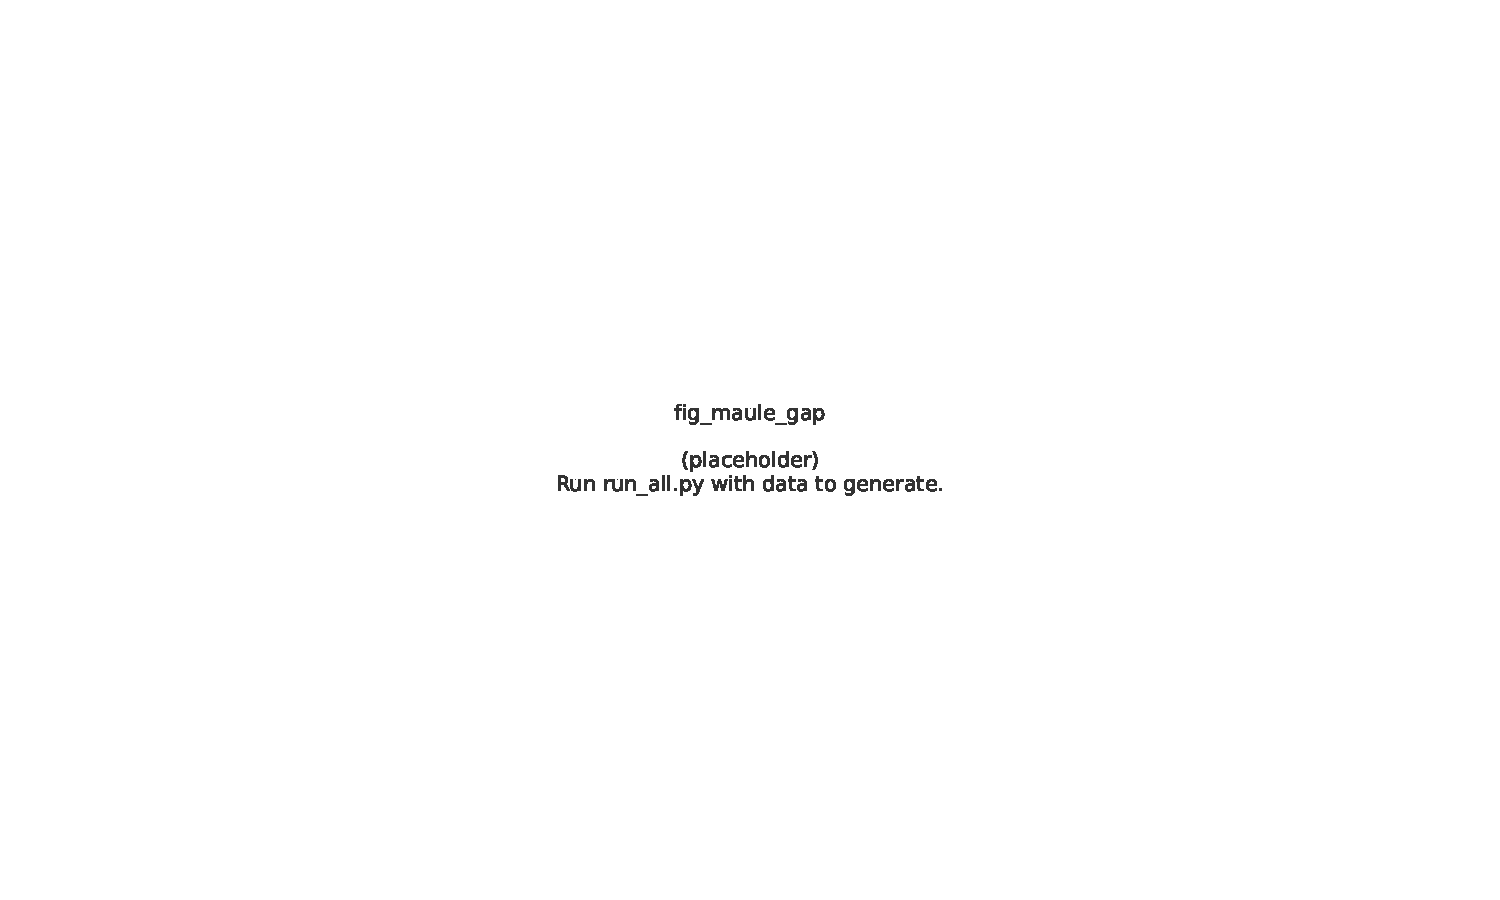
\includegraphics[width=0.85\textwidth]{figures/fig_maule_gap.pdf}
\caption{Maule: Actual $-$ Synthetic GDP per capita.}
\label{fig:maule_gap}
\end{figure}

\end{verbatim}

Replace any placeholder figure paths with the produced files, e.g.:
\begin{verbatim}
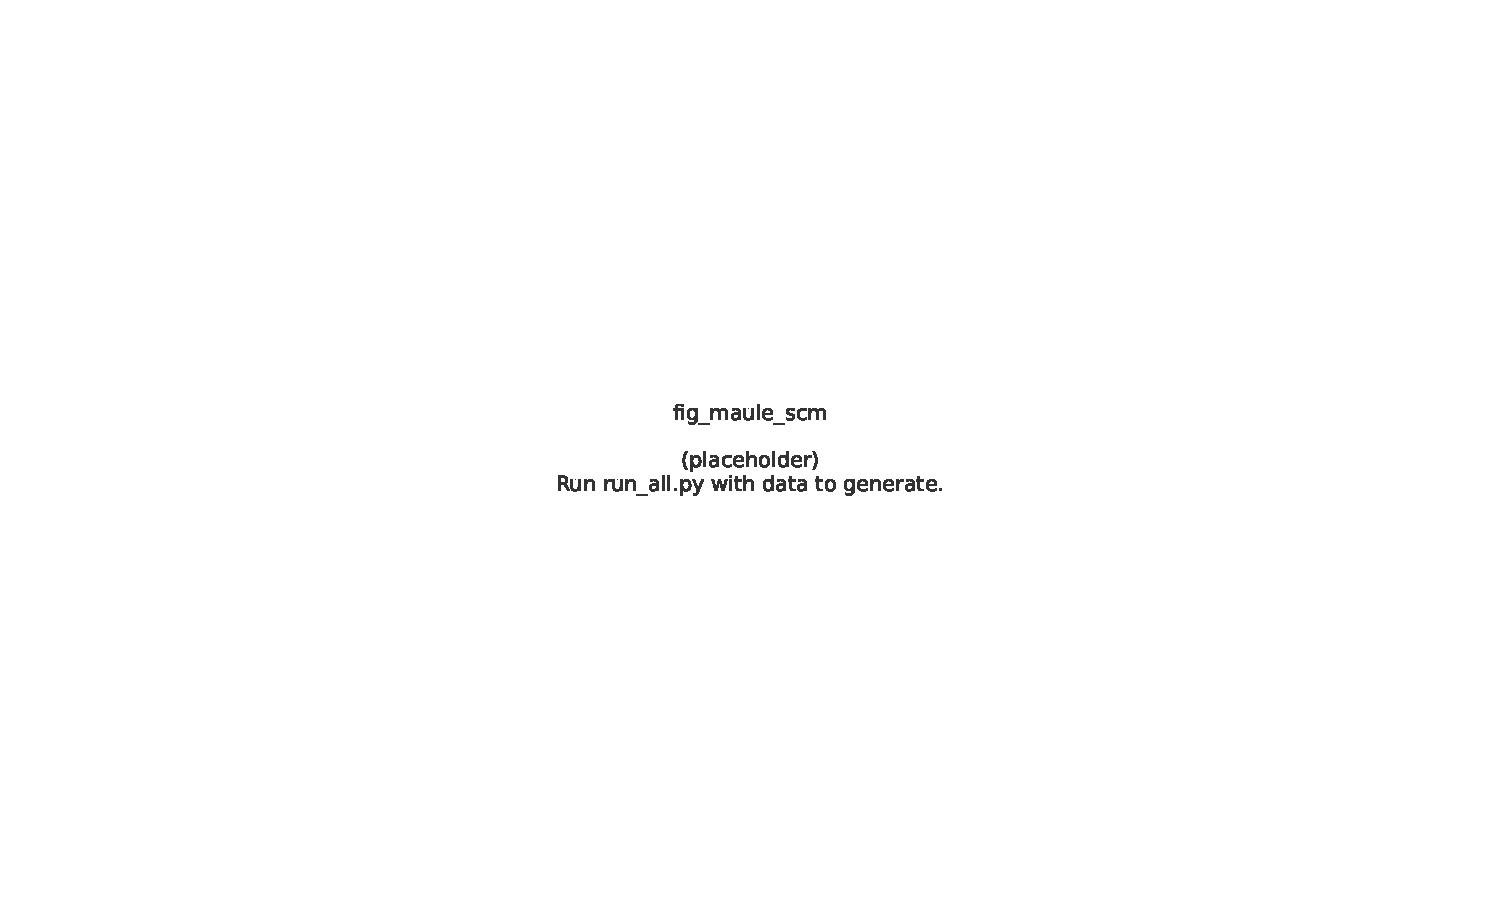
\includegraphics[width=0.8\textwidth]{figures/fig_maule_scm.pdf}
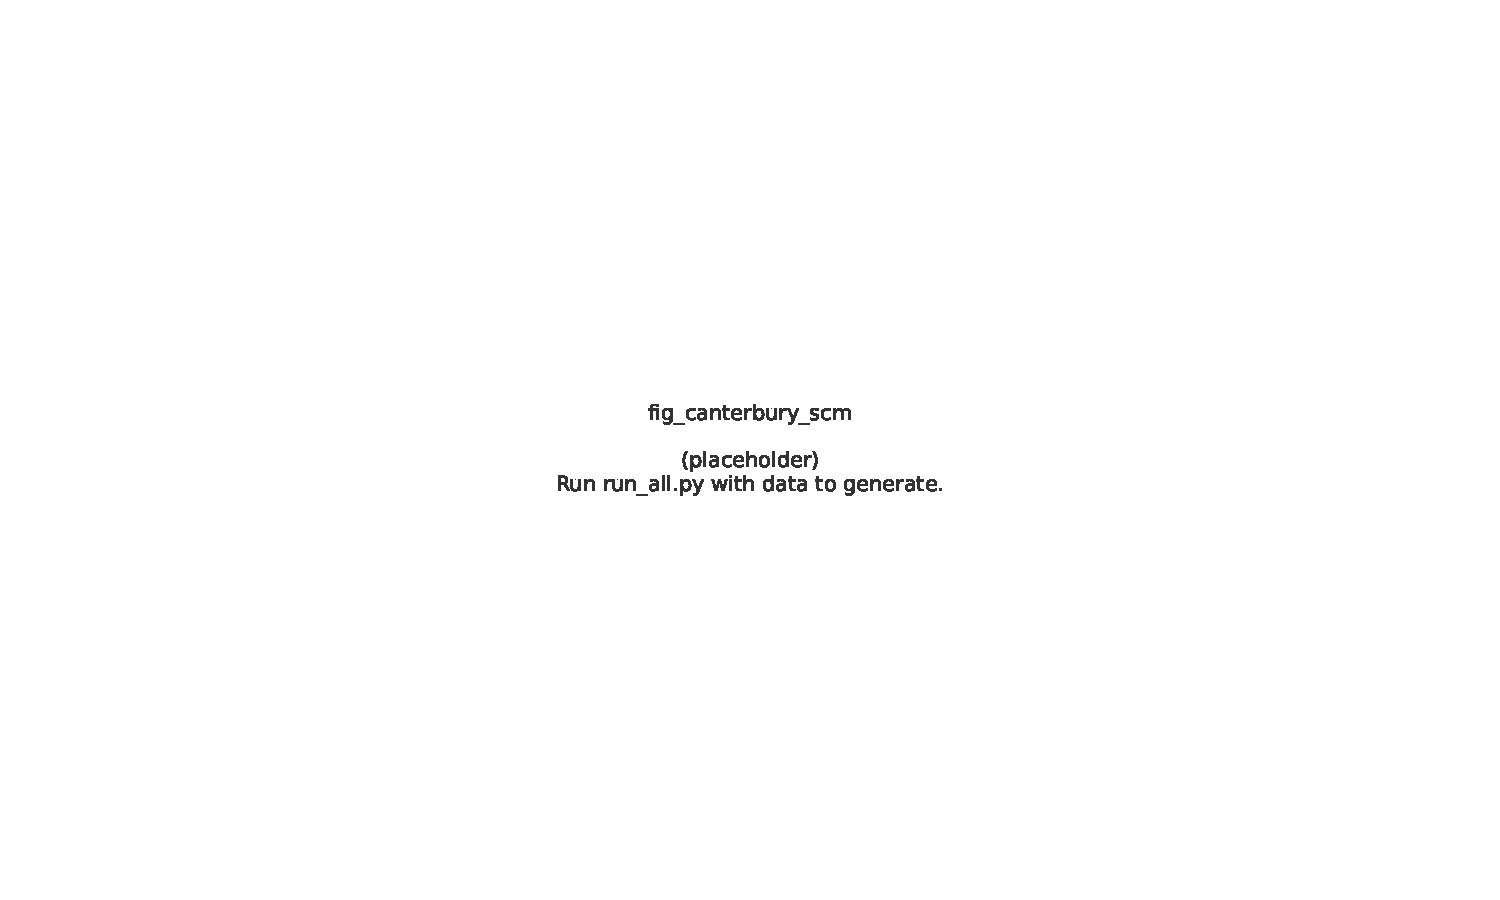
\includegraphics[width=0.8\textwidth]{figures/fig_canterbury_scm.pdf}
\end{verbatim}
